\documentclass[12pt]{article}
\usepackage[utf8]{inputenc}
\usepackage[spanish,es-lcroman, es-tabla]{babel}
\usepackage[autostyle,spanish=mexican]{csquotes}
\usepackage{amsmath}
\usepackage{amssymb}
\usepackage{nccmath}
\numberwithin{equation}{section}
\usepackage{amsthm}
\usepackage{graphicx}
\usepackage{epstopdf}
\DeclareGraphicsExtensions{.pdf,.png,.jpg,.eps}
\usepackage{color}
\usepackage{float}
\usepackage{multicol}
\usepackage{enumerate}
\usepackage[shortlabels]{enumitem}
\usepackage{anyfontsize}
\usepackage{anysize}
\usepackage{array}
\usepackage{multirow}
\usepackage{enumitem}
\usepackage{cancel}
\usepackage{tikz}
\usepackage{circuitikz}
\usepackage{tikz-3dplot}
\usetikzlibrary{babel}
\usetikzlibrary{shapes}
\usepackage{bm}
\usepackage{mathtools}
\usepackage{esvect}
\usepackage{hyperref}
\usepackage{relsize}
\usepackage{siunitx}
\usepackage{physics}
%\usepackage{biblatex}
\usepackage{standalone}
\usepackage{mathrsfs}
\usepackage{bigints}
\usepackage{bookmark}
\spanishdecimal{.}

\setlist[enumerate]{itemsep=0mm}

\renewcommand{\baselinestretch}{1.5}

\let\oldbibliography\thebibliography

\renewcommand{\thebibliography}[1]{\oldbibliography{#1}

\setlength{\itemsep}{0pt}}
%\marginsize{1.5cm}{1.5cm}{2cm}{2cm}


\newtheorem{defi}{{\it Definición}}[section]
\newtheorem{teo}{{\it Teorema}}[section]
\newtheorem{ejemplo}{{\it Ejemplo}}[section]
\newtheorem{propiedad}{{\it Propiedad}}[section]
\newtheorem{lema}{{\it Lema}}[section]

\usepackage[flushleft]{threeparttable}
% \usepackage{mathrsfs}
% \newcommand{\doblederivaday}[1]{#1^{\prime \prime}}
% \newcommand{\derivaday}[1]{#1^{\prime}}
% \newcommand{\dderivadacociente}[2]{\dfrac{d^{2} #1}{d #2^{2}}}
% \newcommand{\derivadacociente}[2]{\dfrac{d {#1}}{d #2}}
% %\renewcommand{\tablename}{Tabla}
% %\newtheorem{defi}{{\it Definición}}[section]
% %\newtheorem{ejemplo}{{\it Ejemplo}}[section]
% %\usepackage{enumerate}
\author{}
\title{Funciones ortogonales \\ {\large Tema 3 - Matemáticas Avanzadas de la Física}\vspace{-3ex}}
\date{ }
\begin{document}
%\renewcommand\theenumii{\arabic{theenumii.enumii}}
\renewcommand\labelenumii{\theenumi.{\arabic{enumii}}}
\maketitle
\fontsize{14}{14}\selectfont
%Notas Arken Capítulo 10 versión djvu
\section{Ecuaciones diferenciales auto-adjuntas.}
Ya hemos abordado y resuelto EDO2, cuya forma general en términos de un operador diferencial lineal de segundo orden ($\mathcal{L}$) es
\begin{equation}
\mathcal{L} u(x) = \left[ p_{0}(x) \, \dv[2]{x} + p_{1}(x) \, \dv{x} + p_{2}(x) \right] \, u(x)
\label{eq:ecuacion_10_01}
\end{equation}
Donde reconocemos que $P(x) = p_{1}(x)/p_{0}(x)$ y $Q(x)= p_{2}(x)/p_{0}(x)$.
\par
%Revisaremos la ecuación diferencial en algún intervalo cerraro $[a,b]$ y que 
Los coeficientes $p_{0}$, $p_{1}$, y $p_{2}$ son funciones reales de $x$ en todo el intervalo $a \leq x \leq b$. Hay que tomar en cuentas un par de condiciones adicionales para las tres funciones:
\begin{enumerate}
\item La función $p_{0}(x)$ es diferente de cero para todo punto en el intervalo abierto $(a,b)$.
\item Las primeras $2-i$ derivadas de la función $p_{i}(x)$ son continuas.
\end{enumerate}
Los ceros de la función $p_{0}(x)$ son puntos singulares de la ecuación diferencial (\ref{eq:ecuacion_10_01}), podemos elegir el intervalo $[a,b]$ de tal manera que no hayan puntos singulares al interior del intervalo, sucede a menudo que los únicos puntos donde pueden existir puntos singulares son los puntos extremos del intervalo: $x = a$ y $x = b$.
\par
Para un operador lineal $\mathcal{L}$, el análogo de una forma cuadrática para una matriz, es la integral
\begin{align}
\begin{aligned}
\matrixel{u}{\mathcal{L}}{u} &\equiv \ip{u}{\mathcal{L} \, u} = \int_{a}^{b} u(x) \, \mathcal{L} \, u(x) \, \dd{u} \\
&= \int_{a}^{b} u \, [ p_{0} \, u^{\prime \prime} + p_{1} \, u^{\prime} + p_{2} \, u ] \, \dd{x}
\end{aligned}
\label{eq:ecuacion_10_02}
\end{align}
donde las primadas de la función real $u(x)$ indican las derivadas. Si cambiamos las derivadas al primer factor, $u$, en la ec. (\ref{eq:ecuacion_10_02}) integrando por partes una o dos veces, nos dirige a la expresión equivalente
\begin{align}
\begin{aligned}
\matrixel{u}{\mathcal{L}}{u} &= [ u(x) \, ( p_{1} - p_{0}^{\prime} ) \, u(x)] \eval_{x=a}^{b} \\
&+ \int_{a}^{b} \left\{ \dv[2]{x} [p_{0} \, u] - \dv{x} [p_{1} \, u] + p_{2} \, u \right\} \, u \, \dd{x}
\end{aligned}
\label{eq:ecuacion_10_03}
\end{align}
Se requiere que las integrales en las ecs. (\ref{eq:ecuacion_10_02}) y (\ref{eq:ecuacion_10_03}) sean idénticas \textbf{para todas las funciones $\bm{u}$ (diferenciables dos veces)}, por lo que los integrandos deben de ser iguales. La comparación nos deja que
\[ u \, (p_{0}^{\prime \prime} - p_{1}) \, u + 2 \, u (p_{0}^{\prime} - p_{1}) \, u^{\prime} = 0 \]
o
\begin{equation}
p_{0}^{\prime} (x) = p_{1} (x)
\label{eq:ecuacion_10_04}
\end{equation}
como ganancia, los valores en los extremos $x=a$ y $x=b$ en la ec. (\ref{eq:ecuacion_10_03}) se anulan.
\par
Por la analogía a la matriz transpuesta, es conveniente definir el operador lineal en la ec. (\ref{eq:ecuacion_10_03})
\begin{align}
\begin{aligned}
\overline{\mathcal{L}} \, u &= \dv[2]{x} [ p_{0} \, u(x)] - \dv{x} [p_{1} \, u(x)] + p_{2} \, u(x) \\
&= p_{0} \dv[2]{u}{x} + \left[ 2 \; p_{0}^{\prime} - p_{1} \right] \; \dv{u}{x} + \left( p_{0}^{\prime \prime} - p_{1}^{\prime} + p_{2} \right) \, u
\label{eq:ecuacion_10_05}
\end{aligned}
\end{align}
Este es el \textbf{operador autoadjunto $\overline{\mathcal{L}}$}.
\par 
Se ha definido el operador autoadjunto $\overline{\mathcal{L}}$ y se ha demostrado que si la ec. (\ref{eq:ecuacion_10_04}) se cumple, entonces $\ip{\overline{\mathcal{L}} \, u}{u} = \ip{u}{\mathcal{L} \, u}$. Siguiendo el mismo procedimiento, podemos mostrar de manera más general que $\ip{v}{\mathcal{L} \, u} = \ip{\mathcal{L} \, v}{u}$. Cuando esta condición se satisface:
\begin{equation}
\setlength{\fboxsep}{3\fboxsep}\boxed{\overline{\mathcal{L}} \, u = \mathcal{L} \, u = \dv{x} \left[ p(x) \dv{u(x)}{x} \right] + q(x) , u(x)}
\label{eq:ecuacion_10_06}
\end{equation}
se dice que $\mathcal{L}$ es un \textbf{operador autoadjunto}. Aquí, para el caso autoadjunto, $p_{0}(x)$ se reemplaza por $p(x)$ y $p_{2}(x)$ por $q(x)$ para evitar subíndices innecesarios.
\par
La forma de la ec. (\ref{eq:ecuacion_10_06}) permite llevar a cabo dos integraciones por partes en la ec. (\ref{eq:ecuacion_10_03}) sin integrados. Toma en cuenta que un operador dado no es inherentemente autoadjunto; su propiedad de autoadjunto depende de las propiedades del espacio en el que actúa la función y en las condiciones de frontera.
\par
Como ejemplos tenemos que la ecuación de Legendre y la ecuación del oscilador lineal son autoadjuntas, pero otras, como las ecuaciones de Laguerre y Hermite, no lo son. Sin embargo, la teoría de las ecuaciones diferenciales autoadjuntas lineales de segundo orden es perfectamente general porque \textbf{siempre podemos transformar} el operador no autoadjunto en la forma autoadjuntada requerida. Considera la ec. (\ref{eq:ecuacion_10_01}) con $p_{0}^{\prime} \neq p_{1}$. Si multiplicamos $\mathcal{L}$ por
\begin{align*}
\dfrac{1}{p_{0}(x)} \exp \left[ \int^{x} \dfrac{p_{1}(t)}{p_{0}(t)} \, \dd{t} \right]
\end{align*}
se obtiene
\begin{align}
\begin{aligned}
\dfrac{1}{p_{0}(x)} \exp \left[ \int^{x} \dfrac{p_{1}(t)}{p_{0}(t)} \dd{t} \right] \, \mathcal{L} \, u(x) &= \dv{x} \left[ \exp \left( \int^{x} \dfrac{p_{1}(t)}{p_{0}(t)} \, \dd{t} \right) \, \dv{u(x)}{x} \right] \\[1em]
&+ \dfrac{p_{2}(x)}{p_{0}(x)} \, \exp \left[ \int^{x} \dfrac{p_{1}(t)}{p_{0}(t)} \, \dd{t} \right] \, u
\end{aligned}
\label{eq:ecuacion_10_07}
\end{align}
que es un operador claramente autoadjunto. Nótese que $p_{0}$ está en el denominador, esto se debe a que necesariamente $p_{0} \neq 0$, en el intervalo $a < x < b$. En el siguiente desarrollo, supondremos que $\mathcal{L}$ ha sido puesto en una forma auto-adjunta.
\section{Funciones propias, valores propios.}
La ecuación de onda de Schrödinger
\begin{align*}
H \, \psi (x) = E \, \psi (x)
\end{align*}
Es el ejemplo más importante de una ecuación de valores propios en física; aquí el operador diferencial $\mathcal{L}$ está definido por el hamiltoniano $H$ y puede que no sea real, y el valor propio se convierte en la energía total $E$ del sistema. La función propia $\psi (x)$ puede ser compleja y generalmente se denomina \textbf{función de onda}. Sobre la base de propiedades de simetría esféricas, cilíndricas o de otro sistema coordenado, una ecuación EDP o de valores propios de tres o cuatro dimensiones, como la ecuación de Schrödinger, puede separarse en ecuaciones de valores propios de una sola variable cada una.
\par
Sin embargo, a veces una ecuación de autovalores toma la forma autoadjunta más general
\begin{equation}
\mathcal{L} \, u(x) + \lambda \, w(x) \, u(x) = 0
\label{eq:ecuacion_10_08}
\end{equation}
donde la constante $\lambda$ es el valor propio y $w(x)$ es una función conocida de peso o densidad; $w(x) > 0$, excepto posiblemente en puntos aislados en los que $w(x) = 0$. Para una elección dada del parámetro $\lambda$, una función $u_{\lambda}(x)$, que satisface la ec. (\ref{eq:ecuacion_10_08}) \textbf{y las CDF impuestas}, se llama una \textbf{función propia} correspondiente a $\lambda$. La constante $\lambda$ es llamada \textbf{valor propio} por los matemáticos.
\par
No hay garantía de que exista una función propia $u_{\lambda} (x)$ para una elección arbitraria del parámetro $\lambda$. De hecho, el requisito de que haya una función propia a menudo restringe los valores aceptables de $\lambda$ en un conjunto discreto. 
\par
El producto interno de dos funciones
\begin{align*}
\ip{v}{u} = \int_{a}^{b} v^{*}(x) \, w(x) \, u(x) \, \dd{x}
\end{align*}
depende de la función de peso y generaliza nuestra definición previa, donde $w(x) = 1$. La función de peso también modifica la definición de \textbf{ortogonalidad} de dos funciones propias: son ortogonales si su producto interno $\ip{u_{\lambda^{\prime}}}{u_{\lambda}} = 0$. La función de peso adicional $w(x)$ aparece a veces como una función de onda asintótica $\psi_{\infty}$ que es un factor común en todas las soluciones de una EDP como la ecuación de Schrödinger, por ejemplo, cuando el potencial $V(x) \to 0$ cuando $x \to \infty$ en $H = T + V$. Podemos encontrar $\psi_{\infty}$ cuando establecemos $V = 0$ en la ecuación de Schrödinger. Otra fuente para $w(x)$ puede ser una barrera de momento angular no nulo $\ell (\ell +1)/x^{2}$ en una EDP o una EDO separada que tiene una singularidad regular y domina en $x \to 0$. En tal caso, la ecuación de índices, muestra que la función de onda tiene a $x^{\ell}$ como factor general. Dado que la función de onda entra dos veces en los elementos de la matriz y las relaciones de ortogonalidad, las funciones de peso en la tabla (\ref{tabla:tabla_01}) provienen de estos factores comunes en ambas funciones de onda radial. Así es como surge el $\exp(-x)$ para los polinomios de Laguerre y $x^{k} \, \exp(-x)$ para los polinomios asociados de Laguerre.
\begin{table}[!ht]
\caption{Tabla con parámetros y coeficientes de ED con valores propios.\label{tabla:tabla_01}}
\centering
\begin{threeparttable}
\begin{tabular}{p{6cm} c c c c }
\hline
\makecell{Ecuación} & $p(x)$ & $q(x)$ & $\lambda$ & $w(x)$ \\ \hline
Legendre & $1 - x^{2}$ & 0 & $\ell (\ell + 1)$ & 1  \\
Asociada de Legendre & $1 - x^{2}$ & 0 & $\ell (\ell + 1)$ & 1  \\
Chebychev I & $(1 - x^{2})^{1/2}$ & $0$ & $n^{2}$ & $(1 - x^{2})^{-1/2}$ \\
Chebychev II & $(1 - x^{2})^{3/2}$ & $0$ & $n^{2}$ & $(1 - x^{2})^{-1/2}$ \\
Ultraesféricos & $(1-x^{2})^{\alpha + 1/2}$ & 0 & $n(n + 2 \alpha)$ & $(1-x^{2})^{\alpha -1/2}$ \\
Bessel$^{b}$, en $0 \leq x \leq a$ & $x$ & $- \dfrac{n^{2}}{x}$ & $a^{2}$ & $x$ \\
Laguerre, en $0 \leq x < \infty$ & $x \; e^{-x}$ & $0$ & $\alpha$ & $e^{-x}$ \\
Asociados de Laguerre & $x^{k+1} \; e^{-x}$ & $0$  & $\alpha - k$ & $x^{k} \; e^{-x}$ \\
Hermite, en $0 \leq x < \infty$ & $e^{-x^{2}}$ & $0$ & $2 \alpha$ & $e^{-x^{2}}$ \\
Oscilador armónico simple & $1$ & $0$ & $n^{2}$ & $1$
\end{tabular}
\begin{tablenotes}
\small
\item $^{a} \: \ell = 0, 1, 2, \ldots, -\ell \leq m < \ell$ son enteros.
\item $^{b} \:$  La ortogonalidad de las funciones de Bessel es bastante especial, como se verá en el desarrollo del Tema 3.
\item $^{c} \: k$ es un entero no negativo.  
\end{tablenotes}
\end{threeparttable}
\end{table}
\newpage
\begin{ejemplo}{\textbf{El deuterón.}}

Para profundizar un poco más en los conceptos de funciones propias y valores propios, consideremos un modelo simple del deuterón.
\par
A partir de experimentos, la energía de enlace es aproximadamente del orden de $\SI{2}{\mega \electronvolt} \ll M \, c^{2} $, con $M = M_{p} = M_{n}$, la masa común de neutrones y protones cuya pequeña diferencia de masa se desprecia. Debido al corto alcance de la fuerza nuclear, las propiedades del deuterón no dependen mucho de la forma detallada del potencial de interacción. Por lo tanto, la interacción nuclear neutrón-protón puede ser modelada por un potencial de pozo cuadrado esféricamente simétrico: 
\begin{equation}
V = \begin{cases}
V_{0} < 0 \hspace{0.5cm} \text{para } 0 \leq r < a \\
V = 0 \hspace{0.5cm} \text{para } r > a
\end{cases}
\end{equation}
La ecuación de onda de Schrödinger es
\begin{equation}
- \dfrac{\hbar^{2}}{M} \laplacian{\psi} + V \, \psi =  E \, \psi
\label{eq:ecuacion_10_10}
\end{equation}
donde el valor propio de energía $E < 0$ para el estado ligado. Para el estado base el momento angular $ \ell = 0$ por que $\ell \neq 0$ es la barrera del momento angular que se agrega. Así, con $\psi =  \psi(r)$, podemos escribir $u(r) = r \, \psi (r)$ podemos representar la ecuación como
\begin{equation}
\dv[2]{u}{r} + k_{1}^{2} \, u = 0
\label{eq:ecuacion_10_11}
\end{equation}
con
\begin{equation}
k_{1}^{2} =  \dfrac{M}{\hbar^{2}} (E - V_{0}) > 0
\label{eq:ecuacion_10_12}
\end{equation}
para el interior de la región $0 \leq r < a$. En la ecuación, $M$ es la masa reducida del sistema protón-neutrón. Para $a < r < \infty$, tenemos
\begin{equation}
\dv[2]{u}{r} - k_{2}^{2} \, u = 0
\label{eq:ecuacion_10_13}
\end{equation}
con
\begin{equation}
k_{2}^{2} = - \dfrac{M \, E}{\hbar^{2}} > 0
\label{eq:ecuacion_10_14}
\end{equation}
La CDF que permite $\psi$ sea finito en $r = 0$, implica que $u(0) = 0$ y
\begin{equation}
u_{1}(r) = \sin k_{1} \, r, \hspace{1.5cm} 0 \leq r < a
\label{eq:ecuacion_10_15}
\end{equation}
Fuera del pozo de potencial, tenemos una combinación lineal de dos exponenciales
\begin{equation}
u_{2}(r) = A \, \exp(k_{2} \, r) + B \exp(-k_{2} \, r) \hspace{1.5cm} a < r < \infty
\label{eq:ecuacion_10_16}
\end{equation}
De la continuidad de la partícula y de la densidad de corriente, hacen que $u_{1}(a) = u_{2}(a)$ y $u^{\prime}_{1}(a) = u^{\prime}_{2}(a)$, éstas condiciones de unión o coincidencia nos dan
\begin{align}
\begin{aligned}
\sin k_{1} \, a &= A \, \exp(k_{2} \, a) + B \, \exp(- k_{2} \, a) \\
k_{1} \, \cos k_{1} \, a &= k_{2} \, A \, \exp(k_{2} \, a) - k_{2} \, B \, \exp(- k_{2} \, a)
\end{aligned}
\label{eq:ecuacion_10_17}
\end{align}
La condición de que nos permite tener una combinación protón-neutrón es tal que
\begin{align*}
\int_{0}^{\infty} u^{2}(r) \dd{r} = 1
\end{align*}
Esta restricción resulta de la imposición en la condición de frontera, la que hace que $\psi(r)$ sea finita mientras $r \to \infty$. Así pues, significa que $A = 0$; al dividir las dos ecuaciones (para cancelar $B$), se obtiene
\begin{equation}
\tan k_{1} \, a = - \dfrac{k_{1}}{k_{2}} = - \sqrt{\dfrac{E - V_{0}}{- E}} 
\label{eq:ecuacion_10_18}
\end{equation}
que es una ecuación relevante para la energía $E$ que tiene un conjunto \emph{discreto} de soluciones:
\begin{enumerate}
\item Si $E$ es tal que satisface la ecuación (\ref{eq:ecuacion_10_18}), las soluciones $u_{1}(r)$ y $u_{2}(r)$ satisfacen las condiciones de frontera.
\item Si la ecuación (\ref{eq:ecuacion_10_18}) no se satisface, \textbf{no existe una solución aceptable}.
\item Los valores de $E$ para los cuales la ecuación (\ref{eq:ecuacion_10_18}) se satisface, corresponde a los valores propios, las funciones $u_{1}$ y $u_{2}$ (o $\psi$) son las funciones propias.
\item En este ejercicio del deuterón, hay un (y sólo un) valor negativo de $E$ que satisface la ecuación (\ref{eq:ecuacion_10_18}), es decir, sólo tiene un estado base.
\end{enumerate}
Pero ¿qué ocurre si $E$ no satisface la ecuación (\ref{eq:ecuacion_10_18})?, es decir, si $E \neq E_{0}$ no es un valor propio.
\par
Gráficamente podemos imaginarnos $E$ y por tanto variar el valor de $k_{1}$ suavemente.
\begin{figure}[!h]
    \centering
    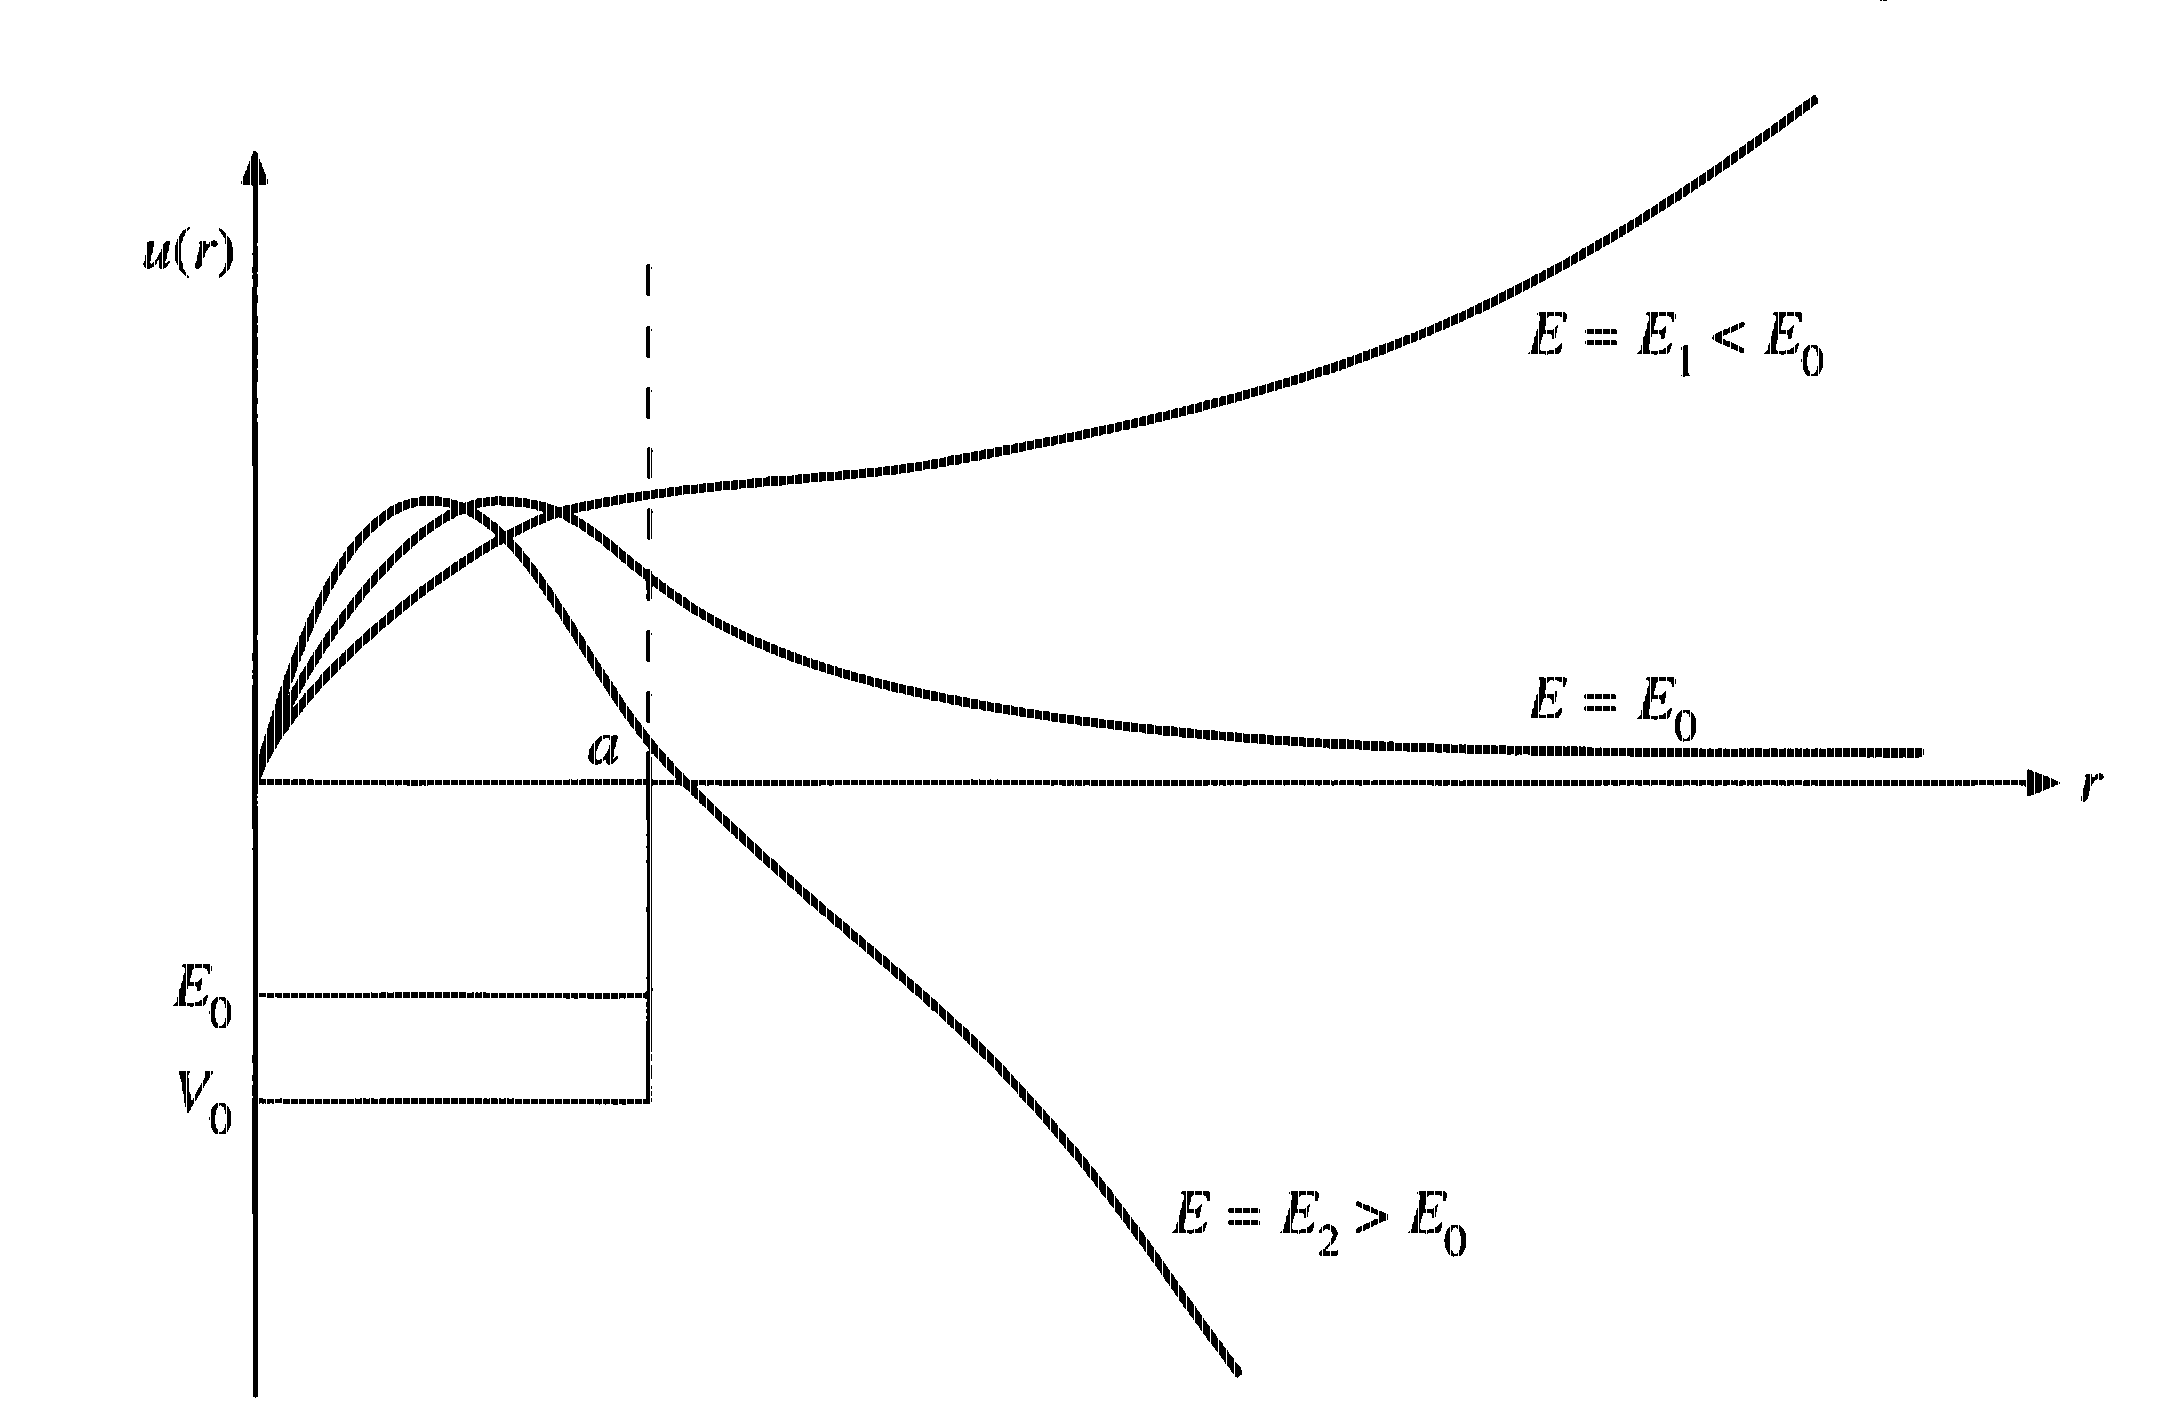
\includegraphics[scale=1.3]{Imagenes/Tema3_01.png}
\caption{Función propia para el deuterón.}
\end{figure}
\begin{itemize}
\item Para $E = E_{1} < E_{0}$, $k_{1}$ disminuye y $\sin k_{1} a$ no ha disminuido lo suficiente para que coincida con $exp(-k_{2} \, a)$. 
\\
Pero las condiciones de unión (ecuación \ref{eq:ecuacion_10_17}), piden que $A > 0$, por lo que la función de onda tiene a $+\infty$ de manera exponencial.
\item Para $E = E_{2} > E_{0}$, $k_{1}$ es grande, y $\sin k_{1} \, a$ tiene rápidamente un pico y luego decae más rápido que $r = a$.
\\
Las condiciones de unión, piden que $A < 0$, por lo que la función de onda tiene a $-\infty$ exponencialmente.
\item Para $E = E_{0}$ un valor propio permite que la función de onda tenga un comportamiento exponencial negativo asintótico.
\end{itemize}
\end{ejemplo}
\section{Condiciones de frontera.}
En la definición anterior de función propia, se observó que la función propia $u_{\lambda} (x)$ era necesaria para satisfacer ciertas CDF impuestas. El término CDF incluye como un caso especial el concepto de condiciones iniciales. Por ejemplo, especificar la posición inicial $x_{0}$ y la velocidad inicial $v_{0}$ en algún problema dinámico, correspondería a las condiciones de frontera de Cauchy. La única diferencia en el uso actual de las CDF en estos problemas unidimensionales es que vamos a aplicar las condiciones en ambos extremos del rango permitido de la variable.
\par
Generalmente, la forma de la ecuación diferencial o las CDF en las soluciones garantizarán que al final de nuestro intervalo (es decir, en el límite, como lo sugiere la ecuación (\ref{eq:ecuacion_10_03})), los siguientes productos se anularán:
\begin{align}
\begin{aligned}
p(x) \, v^{*}(x) \dv{u(x)}{x} \eval_{x = a} = 0 \\[1em]
p(x) \, v^{*}(x) \dv{u(x)}{x} \eval_{x = b} = 0
\label{eq:ecuacion_10_19}
\end{aligned}
\end{align}
Donde $u(x)$ y $v(x)$ son soluciones de la ecuación diferencial (\ref{eq:ecuacion_10_08}). Podemos de cualquier forma, trabajar con un conjunto de CDF menos restrictivas:
\begin{equation}
p(x) \, v^{*}(x) \, \dv{u(x)}{x} \eval_{x = a} = p(x) \, v^{*}(x) \, \dv{u(x)}{x} \eval_{x = b} = 0
\label{eq:ecuacion_10_20}
\end{equation}
en la que $u(x)$ y $v(x)$ son soluciones de la ecuación diferencial correspondiente a valores propios iguales o diferentes. La ecuación (\ref{eq:ecuacion_10_20})) podría satisfacerse si tratáramos con un sistema físico periódico, como el de una red cristalina.
\par
Nótese que se han escrito las ecuaciones anteriores  (\ref{eq:ecuacion_10_19}) y (\ref{eq:ecuacion_10_20}) en términos de $v^{*}(x)$ como conjugado complejo. Cuando las soluciones son reales $v(x) = v^{*}(x)$, podemos omitir el asterisco. En las expansiones exponenciales de Fourier y en ejercicios de mecánica cuántica, las funciones serán complejas y se requiere el conjugado complejo.
\newpage
% \\
% Esas propiedades (ecuaciones \ref{eq:ecuacion_20} y \ref{eq:ecuacion_21}) son importantes para definir el concepto de \emph{Operador Hermitiano}. Una consecuencia de estas condiciones es que el intervalo de integración $(a,b)$ se elige para que éstas condiciones se satisfagan. Si las soluciones son polinomios, los coeficientes $p(x)$ determinarán el rango de integración. Recuerda que también $p(x)$ determina los puntos singulares de la ecuación diferencial. Para soluciones no  polinomiales, por ejemplo, $\sin x$ y $\cos x$, el rango de integración queda determinado por las propiedades de la solución.
\begin{ejemplo}{Elección del intervalo de integración.}

Para $\displaystyle \mathcal{L} = \dv[2]{x}$ una posible ecuación de valores propios es
\begin{equation}
\dv[2]{x} u(x) + n^{2} \, u(x) = 0
\label{eq:ecuacion_10_21}
\end{equation}
con funciones propias
\begin{align*}
u_{n} &= \cos n \, x \\
v_{m} &= \sin m \, x
\end{align*}
La ecuación (\ref{eq:ecuacion_10_20}) es en este caso
\begin{align*}
- n \, \sin m \, x \sin n \, x \eval^{b}_{a} &= 0 \\[1em]
m \, \cos m \, x \, \cos n \, x \eval^{b}_{a} &= 0 
\end{align*}
intercambiando $u_{n}$ y $v_{n}$. Ya que $\sin m \, x$ y $\cos n \, x$ son funciones periódicas, con período $2 \, \pi$ (para $n$ y $m$ $\in \mathbb{N}$), la ecuación (\ref{eq:ecuacion_10_20}) se satisface si $a = x_{0}$ y $b = x_{0} + 2 \, \pi$.
\par
Si un problema prescribe un intervalo diferente, las funciones propias y los valores propios cambiarán junto con las CDF. Las funciones deben elegirse siempre para que se cumplan las CDF (ecuación \ref{eq:ecuacion_10_20}), etc.). Para este caso (series de Fourier) las opciones habituales son $x_{0} = 0$ que conducen al intervalo $(0, 2 \, \pi)$ y $x_{0} = - \pi$, con lo que el intervalo es $(-\pi, \pi)$.
\end{ejemplo}
De aquí y en adelante, el intervalo de ortogonalidad será aquel en donde se cumplan las CDF (ecuación \ref{eq:ecuacion_10_20}).
\par
En la tabla (\ref{tabla:tabla_02}), se enlistan el intervalo de ortogonalidad $[a, b]$ y el factor de peso $w (x)$ para las ecuaciones diferenciales de segundo orden más comunes de la Física Matemática.
\begin{table}[!ht]
\caption{Elección del intervalo de ortogonalidad $[a,b]$ y del factor de peso $\omega(x)$.\label{tabla:tabla_02}}
\centering
\begin{threeparttable}
\begin{tabular}{p{5cm} c c c}
\hline
\makecell{Ecuación} & $a$ & $b$ & $\omega(x)$ \\ \hline
Legendre & $-1$ & $1$ & $1$ \\
Asociados de  Legendre & $-1$ & $1$ & $1$ \\
Chebychev I & $-1$ & $1$ & $(1-x^{2})^{-1/2}$ \\
Chebychev II & $-1$ & $1$ & $(1-x^{2})^{1/2}$ \\
Laguerre & $0$ & $\infty$ & $e^{-x}$ \\
Asociados de Laguerre & $0$ & $\infty$ & $x^{k} e^{-x}$ \\
Hermite & $-\infty$ & $\infty$ & $e^{-x^{2}}$ \\
Oscilador armónico & $0$ & $2 \pi$ & $1$ \\
 & $-\pi$ & $\pi$ & $1$ 
\end{tabular}
\begin{tablenotes}
\small
\item $1.$ El intervalo de ortogonalidad $[a, b]$ está determinado por las CDF.
\item $2.$ La función de peso se presenta a modo de que la EDO queda en una forma auto-adjunta.
\end{tablenotes}
\end{threeparttable}
\end{table}
\section{Operadores Hermitianos.}
Veamos una propiedad importante que se obtiene al combinar un operador diferencial de segundo orden auto-adjunto (ecuación \ref{eq:ecuacion_10_08}) y las soluciones $u(x)$ y $v(x)$, que satisfacen las CDF dadas por la ecuación (\ref{eq:ecuacion_10_20}).
\par
Integramos el producto de $v^{*}$ (conjugado complejo) con el operador diferencial auto-adjunto de segundo orden $\mathcal{L}$ (operando sobre $u$) en el intervalo $a \leq x \leq b$, usando la ecuación, obteniendo:
\begin{equation}
\int_{a}^{b} v^{*} \, \mathcal{L} \, u \, \dd{x} = \int_{a}^{b} v^{*} (p \, u^{\prime})^{\prime} \dd{x} + \int_{a}^{b} v^{*} \, q \, u \, \dd{x}
\label{eq:ecuacion_10_22}
\end{equation}
usando la ecuación (\ref{eq:ecuacion_10_06}). Integrando por partes, obtenemos
\begin{equation}
\int_{a}^{b} v^{*}(p \, u^{\prime})^{\prime} \dd{x} = v^{*} \, p \, u^{\prime} \eval_{a}^{b} - \int_{a}^{b} v^{* \, \prime} \, p \, u^{\prime} \dd{x}
\label{eq:ecuacion_10_23}
\end{equation}
con las CDF, el término integrado se anula cuando se usa la ecuación (\ref{eq:ecuacion_10_20}), al integrar el término que queda, ahora por partes nuevamente, tenemos que
\begin{equation}
- \int_{a}^{b} v^{* \prime} \, p \, u^{\prime} \dd{x} = - v^{* \, \prime} \, p \, u \eval_{a}^{b} + \int_{a}^{b} u(p \, v^{* \, \prime})^{\prime} \dd{x}
\label{eq:ecuacion_10_24}
\end{equation}
El término integrado se anula nuevamente al considerar la ecuación (\ref{eq:ecuacion_10_20}). Una combinación de las ecuaciones (\ref{eq:ecuacion_10_22}) a la (\ref{eq:ecuacion_10_24}), nos resulta en
\begin{equation}
\int_{a}^{b} v^{*} \, \mathcal{L} \, u \, \dd{x} = \int_{a}^{b} u (\mathcal{L}  \, v)^{*} \dd{x}
\label{eq:ecuacion_10_25}
\end{equation}
Esta propiedad nos dice que el operador $\mathcal{L}$ es Hermitiano respecto a las funciones $u(x)$ y $v(x)$, las cuales satisfacen las CDF que se especifican por la ecuación (\ref{eq:ecuacion_10_20}).
\section{Operadores Hermitianos en mecánica cuántica.}
Generalizando la teoría de operadores Hermitianos en mecánica cuántica, podemos agregar que: los operadores no necesitan ser operadores de segundo orden y ni ser reales. $\displaystyle p_{x} = - i \, \hbar(\pdv{x})$ sería un operador Hermitiano.
\par
Simplemente asumimos (como es habitual en la mecánica cuántica) que las funciones de onda satisfacen las CDF apropiadas: se anulan con la fuerza suficiente en el infinito o tienen un comportamiento periódico (como en una red cristalina, o la intensidad de la unidad para problemas de dispersión). 
\par
El operador $\mathcal{L}$ se llama Hermitiano si
\begin{equation}
\setlength{\fboxsep}{3\fboxsep}\boxed{\int \psi_{1}^{*} \, \mathcal{L} \, \psi_{2} \dd{\tau} =  \int (\mathcal{L} \, \psi_{1})^{*} \, \psi_{2} \dd{\tau}}
\label{eq:ecuacion_10_26}
\end{equation}
El adjunto $A^{\dagger}$ de un operador $A$ se define como 
\begin{equation}
\setlength{\fboxsep}{3\fboxsep}\boxed{\int \psi_{1}^{*} \, A^{\dagger} \, \psi_{2} \dd{\tau} \equiv \int (A \, \psi_{1})^{*} \, \psi_{2} \dd{\tau}}
\label{eq:ecuacion_10_27}
\end{equation}
Esto generaliza nuestra definición clásica del operador diferencial de segundo orden, ec. (\ref{eq:ecuacion_10_05}). El operador adjunto está definido en términos del resultado de la integral, con $A^{\dagger}$ como parte del integrando. Si $A = A^{\dagger}$ (\textbf{auto-adjunto}), entonces $A$ es Hermitiano. %Al revés no es tan sencillo (y no siempre cierto), pero en mecánica cuántica los términos \emph{auto-adjunto} y \emph{Hermitiano}, se usan como sinónimos.
\par
El \textbf{valor esperado} de un operador $\mathcal{L}$ se define como
\begin{equation}
\setlength{\fboxsep}{3\fboxsep}\boxed{\expval{\mathcal{L}} = \int \psi^{*} \, \mathcal{L} \, \psi \dd{\tau}}
\label{eq:ecuacion_10_28a}
\end{equation}
En el ámbito de mecánica cuántica $\expval{\mathcal{L}}$ corresponde al resultado de una medición de una cantidad física representada por $\mathcal{L}$ donde el sistema físico es un estado descrito por la función de onda $\psi$. Si queremos que $\mathcal{L}$ sea Hermitiano, debemos de mostrar que $\expval{\mathcal{L}}$ es real (en correspondencia de una medición en física). Tomando el conjugado complejo de la ecuación (\ref{eq:ecuacion_10_28a}), tenemos
\begin{align*}
\expval{\mathcal{L}}^{*} &= \left[ \int \psi^{*} \, \mathcal{L} \, \psi \dd{\tau} \right] = \int \psi \, \mathcal{L}^{*} \, \psi^{*} \dd{\tau}
\end{align*}
Ordenando los factores en el integrando, resulta
\begin{align*}
\expval{\mathcal{L}}^{*} = \int (\mathcal{L} \, \psi)^{*} \, \psi \dd{\tau}
\end{align*}
De la definición de operador Hermitiano (ecuación \ref{eq:ecuacion_10_26})
\begin{equation}
\expval{\mathcal{L}}^{*} = \int \psi^{*} \, \mathcal{L} \, \psi \dd{\tau} = \expval{\mathcal{L}} 
\label{eq:ecuacion_10_28b}
\end{equation}
o $\expval{\mathcal{L}}$ es real. Vale la pena señalar que $\psi$ no es necesariamente una función propia de $\mathcal{L}$.
\section{Operadores Hermitianos.}
Los operadores Hermitianos o auto-adjuntos tienen tres propiedades de gran importancia en la física tanto clásica como cuántica:
\begin{enumerate}
\item Los valores propios son reales.
\item Cuenta con un conjunto de funciones propias ortogonales.
\item Las funciones propias forman un conjunto completo.
\par
Esta tercera propiedad no es universal. Se mantiene para los operadores diferenciales lineales de segundo orden en forma de Sturm-Liouville (autoadjunto).
\end{enumerate}
\subsection{Valores propios reales.}
Sea
\begin{equation}
\mathcal{L} \, u_{i} + \lambda_{i} \, w \, u_{i} = 0
\label{eq:ecuacion_10_29}
\end{equation}
Suponemos la existencia de un segundo valor propio y función propia
\begin{equation}
\mathcal{L} \, u_{j} + \lambda_{j} \, w \, u_{j} = 0
\label{eq:ecuacion_10_30}
\end{equation}
Entonces, al tomar el conjugado completo, resulta
\begin{equation}
\mathcal{L}^{*} \, u_{j}^{*} + \lambda_{j}^{*} \, w \, u_{j}^{*} = 0
\label{eq:ecuacion_10_31}
\end{equation}
donde $w(x) \geq 0$ es una función real. Permitimos que tanto $\lambda_{k}$ que son los valores propios, así como $u_{k}$ las funciones propias, sean complejos. Multiplicando la ecuación (\ref{eq:ecuacion_10_29}) y (\ref{eq:ecuacion_10_31}) por $u_{i}$, y luego las restamos, se obtiene
\begin{equation}
u_{j}^{*} \, \mathcal{L} \, u_{i} - u_{i} \mathcal{L}^{*} \, u_{j}^{*} =  (\lambda_{j}^{*} - \lambda_{i}) \, w \, u_{i} \, u_{j}^{*}
\label{eq:ecuacion_10_32}
\end{equation}
integramos en el intervalo $a \leq x \leq b$,
\begin{equation}
\int_{a}^{b} u_{j}^{*} \, \mathcal{L} \, u_{i} \dd{x} - \int_{a}^{b} u_{i} \, \mathcal{L}^{*} \, u_{j}^{*} \dd{x} = (\lambda_{j}^{*} - \lambda_{i}) \, \int_{a}^{b}  u_{i} \, u_{j}^{*} \, w \dd{x}
\label{eq:ecuacion_10_33}
\end{equation}
Como $\mathcal{L}$ es Hermitiano, el lado izquierdo de la igualdad se anula, considerando la ecuación (\ref{eq:ecuacion_10_26}) y tenemos
\begin{equation}
(\lambda_{j}^{*} - \lambda_{i}) \, \int_{a}^{b}  u_{i} \, u_{j}^{*} \, w \dd{x} = 0
\label{eq:ecuacion_10_34}
\end{equation}
Si $i=j$ la integral no se puede anular ($w(x) > 0$ para puntos aislados), a menos que tengamos el caso trivial $u_{i} = 0$. Por tanto el coeficiente $(\lambda_{i}^{*} - \lambda_{j})$ debe de ser cero
\begin{equation}
\lambda_{i}^{*} = \lambda_{i}
\label{eq:ecuacion_10_35}
\end{equation}
Lo que es una prueba matemática de que el valor propio es real, ya que $\lambda_{i}$ representa a cualquiera de los valores propios, se cumple esta propiedad.
\par
En mecánica cuántica los valores propios corresponden a cantidades medibles, tales como la energía o el momento angular. Con la teoría revisada en términos de operadores Hermitianos, esta prueba de que los valores propios nos garantiza que la teoría predice valores reales para esas cantidades físicas medibles.
% \subsection{Funciones propias ortogonales.}
% Si tomamos $i \neq	j$ y si $\lambda_{i} \neq \lambda_{j}$ la integral del producto de dos funciones propias diferentes debe de anularse:
% \begin{equation}
% \int_{a}^{b} u_{i}u*_{j} w dx = 0
% \label{eq:ecuacion_35}
% \end{equation}
% Esta condición es llamada \emph{ortogonalidad}. Se dice que las funciones propias $u_{i}(x)$ y $u_{j}(x)$ son ortogonales con respecto a una función de peso $w(x)$ en el intervalo $[a,b]$.
% \\
% Si tenemos el caso $i \neq j$ pero se mantiene que $\lambda_{i} = \lambda_{j}$, se tiene el llamado caso \emph{degenerado}. Esto significa que la independencia linea de las funciones propias que corresponden al mismo valor propio, no son automáticamente ortogonales, por lo que deberíamos usar un método que nos permita recuperar el conjunto ortogonal.  Aunque tengamos funciones propias en el caso degenerado y sean no ortogonales, siempre se pueden ortogonalizar.
% \\
% \textbf{Ejemplo: Series de Fourier.}
% \\
% Consideremos la ecuación 
% \[ \dfrac{d^{2}}{d x^{2}} y(x) + n^{2} y(x) = 0 \]
% Que en mecánica cuántica puede describir una partícula en una caja, o puede representar la cuerda de un violín con funciones propias (degeneradas) $\cos nx, \sin nx$.
% \\
% Con $n$ real, las integrales ortogonales son
% \begin{enumerate}[label=\alph*)]
% \item $\begin{aligned}[t] \int_{x_{0}}^{x_{0} +  2 \pi} \sin mx \sin nx dx = C_{n} \delta_{nm} \end{aligned} $ 
% \item $\begin{aligned}[t] \int_{x_{0}}^{x_{0} +  2 \pi} \cos mx \cos nx dx = D_{n} \delta_{nm} \end{aligned} $ 
% \item $\begin{aligned}[t] \int_{x_{0}}^{x_{0} +  2 \pi} \sin mx \cos nx dx = 0 \end{aligned} $
% \end{enumerate}
% Para un intervalo de $2 \pi$ el análisis previo, garantiza la delta de Kronecker en los incisos a) y b), pero no para el iniciso c), ya que c) involucra funciones propias degeneradas. Pero vemos que en c) siempre se anula para todas las integrales $m$ y $n$.
% \\
% De la teoría de Sturm-Liouville no nos dice nada sobre los valores de $C_{n}$ y $D_{n}$. Al calcularlos:
% \begin{eqnarray*}
% C_{n} &= \begin{cases}
% \pi  & n \neq 0 \\
% 0  & n = 0 \end{cases}  \nonumber \\
% D_{n} &= \begin{cases}
% \pi & n \neq 0 \\
% 2 \pi & n = 0 \end{cases}
% \end{eqnarray*}
% La ortogonalidad de los integrandos forma la base para las series de Fourier.
% \\
% \textbf{Ejemplo: Expansión de funciones propias ortogonales: una onda cuadrada.}
% \\
% La propiedad de \emph{completez} significa que cierta clase de funciones (funciones continuas por secciones o pedazos), puede representarse por una serie de funciones propias ortogonales, con cualquier grado de precisión. Consideremos la onda cuadrada:
% \begin{equation}
% f(x) = \begin{cases}
% \dfrac{h}{2} & 0 < x < \pi \\
% - \dfrac{h}{2} & -\pi < x < o
% \end{cases}
% \label{eq_ecuacion_36}
% \end{equation}
% Esta función puede desarrollarse en funciones propias de varios tipos: Legendre, Hermite, Chebyshev, etc. La elección de la función propia se hace en base a la conveniencia del problema. Si elegimos para el desarrollo de la solución, las funciones propias $\cos nx$ y $\sin nx$.
% \\
% La serie de funciones propias se escribe conveniente (y convencionalmente) como
% \[ f(x) = \dfrac{a_{0}}{2} + \sigma_{n=1}^{\infty} (a_{n} \cos nx +  b_{n} \sin nx) \]
% De la ortogonalidad de los integrados, los coeficientes están dados por
% \begin{eqnarray*}
% a_{n} = \dfrac{1}{\pi} \int_{-\pi}^{\pi} f(t) \cos nt dt \\
% b_{n} = \dfrac{1}{\pi} \int_{-\pi}^{\pi} f(t) \sin nt dt, \hspace{1cm} n = 0,1,2,\ldots
% \end{eqnarray*}
% La sustitición directa de $\pm h/2$ para $f(t)$, devuelve que
% \[ a_{n} = 0 \]
% lo que ya se esperaba dada la antisimetría y además
% \[ b_{n} = \dfrac{h}{n \pi} (1 - \cos n \pi) = \begin{cases}
% 0 & n \text{ par} \\
% \dfrac{2h}{n \pi} & n \text{ impar} \end{cases} \]
% Por lo que la expansión de las funciones propias (de Fourier) de una onda cuadrada es
% \begin{equation}
% f(x) = \dfrac{2h}{\pi} \sum_{n=0}^{\infty} \dfrac{\sin(2n+1)x}{(2n+1)}
% \end{equation}
% \subsection{Degeneración.}
% Si $N$ funciones propias linealmente independientes corresponden al mismo valor propio, se dice que el valor propio es $N$-veces degenerado.
% \\
% Un ejemplo directo lo tomamos de las funciones propias y valores propios en la ecuación del oscilador lineal: para cada valor propio $n$, hay dos posibles soluciones: $\sin x$ y $\cos x$ (y cualquier posibles combinación lineal). En este caso, las funciones son degeneradas o el valor propio es degenerado.
% \\
% Otro ejemplo es el sistema electrón en un átomo (no relativista y omitiendo el spin). De la ecuación de Schrödinger para el hidrógeno
% \[ - \dfrac{\hbar^{2}}{2m} \nabla^{2} \psi - \dfrac{Z e^{2}}{r} \psi =  E \psi \]
% la energía total del electrón es el valor propio.
% \\
% Si nombramos $E_{nLM}$ usando los números cuánticos $n$, $L$ y $M$ como subíndices. Para cada diferente conjunto de números cuánticos $(n,L.M)$ existe una función propia linealmente independiente $\psi_{nLM}(r,\theta, \varphi)$.
% \\
% Para el hidrógeno, la energía $E_{nLM}$ es independiente de $L$ y $M$. Con $0 \leq L \leq n-1$ y $-L \leq M \leq L$, el valor propio es $n^{2}$-veces degenerado (que al incluir el espín del electrón, lo elevaría a $2n^{2}$)
% \\
% En átomos con más de un electrón, el campo electrostático no es mayor a un potencial de tipo $r^{-1}$. La energía depende de $L$ como de $n$, pero no de $M$. En este caso, la energía $E_{nLM}$ es aún $(2L+1)$-veces degenerada. Esta particularidad se puede remover al aplicar un campo magnético externo, dando origen al efeto Zeeman.
\newpage
\section{Ortogonalización de Gram-Schmidt.}
Este método toma un conjunto de funciones linealmente dependientes no ortogonales y genera un conjunto ortogonal en un intervalo arbitrario con respecto a una función de peso arbitraria.
\par
Veamos el caso de la normalización de funciones, que implica lo siguiente:
\[ \int_{a}^{b} \varphi_{i}^{2} \, w \, \dd x  =  N_{i}^{2} \]
revisemos que no se le ha puesto atención al valor de $N_{i}$. Ya que la ecuación básica (ec. (\ref{eq:ecuacion_10_08}) es lineal y homogénea, podemos multiplicar la solución por cualquier constante, de tal manera que sigue siendo solución. Por lo que podemos pedir que tal solución $\varphi_{i}(x)$ se multiplique por $N_{i}^{-1}$ y ahora la nueva $\varphi_{i}$ (normalizada) satisface
\begin{equation}
\int_{a}^{b} \varphi_{i}^{2} (x) \, w(x) \, \dd x = 1
\label{eq:ecuacion_10_39}
\end{equation}
o en términos de una delta
\begin{equation}
\int_{a}^{b} \varphi_{i}(x) , \varphi_{j} (x) , w(x) \, \dd x = \delta_{ij}
\label{eq:ecuacion_10_40}
\end{equation}
La ecuación (\ref{eq:ecuacion_10_39}) nos dice que hemos normalizado a la unidad; incluyendo la propiedad de ortogonalidad, tenemos la ecuación (\ref{eq:ecuacion_10_40}), las funciones que las satisfacen, se dice que son \textbf{ortonormales} (ortogonales y normalizadas), cabe señalar que existen otras formas de normalización.
\par
Consideremos tres conjuntos de funciones:
\begin{enumerate}
\item Un conjunto original, linealmente independiente $u_{n}(x)$ con $n=0,1,2,\ldots$
\item Un conjunto ortogonal $\psi_{n}(x)$ que se va a construir.
\item Un conjunto de funciones $\varphi_{n}(x)$ que será nnormalizadas $\psi_{n}(x)$
\end{enumerate}
Tendremos las siguientes propiedades
\begin{center}
{\fontsize{12}{12}\selectfont
\begin{tabular}{l l l}
    
\hline
$u_{n}(x)$ & $\psi_{n}(x)$ & $\varphi_{n}(x)$ \\ \hline
linealmente independiente &    linealmente independiente & linealmente independiente \\
no ortogonal & ortogonal & ortogonal \\
no  normalizada & no normalizada & normalizada \\
 & & (ortonormal)
\end{tabular}
}
\end{center}

La técnica de Gram-Schmidt consiste en tomar la $n-\psi$-función $(\psi_{n}$) que sea $u_{n}(x)$ más un combinación lineal no conocida de la función $\varphi$ previa. El que haya una nueva $u_{n}(x)$ nos dará la garantía de que se mantenga la independencia lineal.

El que $\psi_{n}(x)$ sea ortogonal para cada $\varphi$ previa, apenas nos da elementos para determinar los coeficientes desconocidos. Así cuando ya se determine $\psi_{n}$, se normaliza a la unidad, dejando $\varphi_{n}(x)$. Este procedimiento se repite para las $\psi_{n+1}(x)$.

Empezamos con $n=0$, sea
\begin{equation}
\psi_{0} = u_{0}(x)
\label{eq:ecuacion_10_41}
\end{equation}
no nos preocupemos al no tener una $\varphi$ previa. Entonces normalizamos
\begin{equation}
\varphi_{0}(x) = \dfrac{\psi_{0}(x)}{\left[ \int \psi_{0}^{2} \, w \, \dd x \right]^{1/2}}
\label{eq:ecuacion_10_42}
\end{equation}
Para $n=1$, tenemos
\begin{equation}
\psi_{1}(x) = u_{1}(x) + a_{1,0} \, \varphi_{0}(x)
\label{eq:ecuacion_10_43}
\end{equation}
Que requiere que $\psi_{1}(x)$ sea ortogonal a $\varphi_{0}(x)$, con esto se conduce a
\begin{equation}
\int \psi_{1} \, \varphi_{0} \, w \, \dd x = \int u_{1} \, \varphi_{0} \, w \, \dd x + a_{1,0} \int \varphi_{0}^{2} \, w \,  \dd x = 0
\label{eq:ecuacion_10_44}
\end{equation}
Ya que $\varphi_{0}$ se normaliza a la unidad (ec. \ref{eq:ecuacion_10_42}), tenemos
\begin{equation}
a_{1,0} = - \int	u_{1} \, \varphi_{0} \, w \, \dd x
\label{eq:ecuacion_10_45}
\end{equation}
fijando el valor de $a_{1, 0}$. Normalizando, definimos
\begin{equation}
\varphi_{1} (x) = \dfrac{\psi_{1}(x)}{\left( \int \psi_{1}^{2} \, w \, \dd x \right)^{1/2}}
\label{eq:ecuacion_10_46}
\end{equation}
Generalizando, resulta
\begin{equation}
\varphi_{i}(x) = \dfrac{\psi_{i}(x)}{\left( \int \psi_{i}^{2}(x) \, w(x) \, \dd x \right)^{1/2}}
\label{eq:ecuacion_10_47}
\end{equation}
donde
\begin{equation}
\psi_{i}(x) = u_{i} + a_{1,0} \, \varphi_{0} + a_{i,1} \, \varphi_{1} + \ldots + a_{i,i-1} \, \varphi_{i-1}
\label{eq:ecuacion_10_48}
\end{equation}
Los coeficientes $a_{i, j}$ están dados por
\begin{equation}
a_{i, j} = - \int u_{i} \, \varphi_{j} \, w \, \dd x
\label{eq:ecuacion_10_49}
\end{equation}
La ecuación (\ref{eq:ecuacion_10_49}) es para una normalización unitaria. Para otros tipos de normalización, se tiene que
\[ \int_{a}^{b} \left[ \varphi_{j} (x) \right]^{2} \, w(x) \, \dd x =  N_{j}^{2} \]
La ecuación (\ref{eq:ecuacion_10_47}) se re-emplaza por
\begin{equation}
\varphi_{i}(x) =  N_{i} \: \dfrac{\psi_{i}(x)}{\left( \int \psi_{i}^{2} \, w \, \dd x \right)^{1/2}}
\label{eq:ecuacion_10_47a}
\end{equation}
y los términos $a_{i,j}$ resultan
\begin{equation}
a_{i, j} = - \dfrac{\int u_{i} \, \varphi_{j} \, w \, \dd x}{N_{j}^{2}}
\label{eq:ecuacion_10_49a}
\end{equation}
Las ecuaciones (\ref{eq:ecuacion_10_48}) y (\ref{eq:ecuacion_10_49}) pueden escribirse en términos de operadores de proyección $P_{j}$. Si consideramos que $\varphi_{n}(x)$ forman un espacio vectorial lineal, la integral en la ecuación \ref{eq:ecuacion_10_49}) puede interpretarse como la proyección de $u_{i}$ en la \enquote{coordenada} $\varphi_{j}$ o la componente $j$-ésima de $u_{i}$. Con
\[ P_{j} \, u_{i}(x) = \left[ \int u_{i}(t) \, \varphi_{j}(t) \, w(t) \right] \varphi_{j}(x) \]
la ecuación (\ref{eq:ecuacion_10_48}) resulta ahora
\begin{equation}
\psi_{i}(x) = \left\{ 1 - \sum_{j=1}^{i-1} P_{j} \right\} u_{i}(x)
\label{eq:ecuacion_10_48a}
\end{equation}
Restando los $j-$-ésimos compoenentes: $j=1$ a $i-1$, resulta que $\psi_{i}(x)$ es ortogonal para todo $\varphi_{j}(x)$.
\par
 Cabe señalar que el procedimiento de Gram-Schmidt es una manera de construir un conjunto ortogonal o ortonormal, pero las funciones $\varphi_{i}(x)$ no son únicas. Existe un infinito de posibles conjuntos ortonormales para un intervalo dado y una función de peso dada.
\begin{ejemplo} \textbf{Ejemplo: Ortogonalización de Gram-Schmidt para los polinomios de Legendre.}
Queremos generar un conjunto ortonormal a partir de las funciones $u_{n}(x)=x^{n}$, $n=0,1,2,\ldots$. El intervalo es $-1 \leq x \leq 1$ y la función de peso es $w(x)=1$.

De acuerdo a la técnica descrita de ortogonaliación de Gram-Schmidt
\begin{equation}
u_{0} = 1 \hspace{1.5cm} \varphi_{0} =  \dfrac{1}{\sqrt{2}}
\label{eq:ecuacion_10_50}
\end{equation}
Entonces
\begin{equation}
\psi_{1}(x) = x + a_{1,0} \dfrac{1}{\sqrt{2}}
\label{eq:ecuacion_10_51}
\end{equation}
donde
\begin{equation}
a_{1, 0} = - \int_{-1}^{1} \dfrac{x}{\sqrt{2}} \, \dd x = 0
\label{eq:ecuacion_10_52}
\end{equation}
por simetría. Normalizando $\psi_{1}$, obtenemos
\begin{equation}
\varphi_{1}(x) = \sqrt{\dfrac{3}{2}} \, x
\label{eq:ecuacion_10_53}
\end{equation}
Continuando el método de Gram-Schmidt, se define ahora
\begin{equation}
\psi_{2} (x) = x^{2} +  a_{2, 0} \dfrac{1}{\sqrt{2}} +  a_{2, 1} \sqrt{\dfrac{3}{2}} \, x
\label{eq:ecuacion_10_54}
\end{equation}
donde
\begin{align}
a_{2, 0} &= - \int_{-1}^{1} \dfrac{x^{2}}{\sqrt{2}} \, \dd x = - \dfrac{\sqrt{2}}{3} \label{eq:ecuacion_10_55} \\[1em] 
a_{2, 1} &= - \int_{-1}^{1} \sqrt{\dfrac{3}{2}} \, x^{3} \dd x = 0 \label{eq:ecuacion_10_56}
\end{align}

\end{ejemplo}
de nueva cuenta por simetría. Por tanto
\begin{equation}
\psi_{2}(x) = x^{2} - \dfrac{1}{3}
\label{eq:ecuacion_10_57}
\end{equation}
normalizando a la unidad, tenemos
\begin{equation}
\varphi_{2} (x) = \sqrt{\dfrac{5}{2}} \, \dfrac{1}{2} \, (3 x^{2} - 1)
\label{eq:ecuacion_10_58}
\end{equation}
La siguiente función $\varphi_{3}(x)$ es
\begin{equation}
\varphi_{3} (x) = \sqrt{\dfrac{7}{2}} \, \dfrac{1}{2} \, (5 x^{3} - 3x)
\label{eq:ecuacion_10_59}
\end{equation}
Se puede demostrar que
\begin{equation}
\varphi_{n}(x) = \sqrt{\dfrac{2n+1}{2}} \, P_{n}(x)
\label{eq:ecuacion_59}
\end{equation}
donde $P_{n}$ es el polinomio de orden $n$ de Legendre.
\subsection{Polinomios ortogonales.}
El ejemplo anterior se ha elegido estrictamente para ilustrar el procedimiento de Gram-Schmidt. Aunque tiene la ventaja de introducir los polinomios de Legendre, las funciones iniciales $u_{n} = x^{n}$ no son funciones propias degeneradas y no son soluciones de la ecuación de Legendre. Son simplemente un conjunto de funciones que hemos reorganizado aquí para crear un conjunto ortonormal para el intervalo dado y la función de peso dada. El hecho de que hayamos obtenido los polinomios de Legendre no es una magia negra, sino una consecuencia directa de la elección de la función de peso y del intervalo.
\par
\begin{table}[H]
\resizebox{\textwidth}{!}{%
\begin{tabular}{p{3cm} c c l}
\hline
Polinomios & Intervalo & $w(x)$ & Normalización estándar \\ \hline
Legendre & $ -1 \leqq x \leq 1$ & $1$ & $ \int_{-1}^{1} \left[ P_{n}(x) \right]^{2} dx = \dfrac{2}{2n+1} $ \\
Modificados de Legendre & $ 0 \leq x \leq 1$ & $1$ & $ \int_{-1}^{1} \left[ P_{n}^{*}(x) \right]^{2} dx = \dfrac{2}{2n+1} $ \\
Chebyshev I & $-1 \leq x \leq 1$ & $(1-x^{2})^{-1/2}$ & $ \int_{-1}^{1} \left( T_{n}(x) \right)^{2}(1-x^{2})^{-1/2} dx = \begin{cases} 
\frac{\pi}{2} & n \neq 0 \\
\pi & n = 0 \end{cases} $ \\
Chebyshev II & $-1 \leq x \leq 1$ & $(1-x^{2})^{1/2}$ & $\int_{-1}^{1} [U_{n} (x)]^{2} \, (1-x^{2})^{1/2} \, \dd x = \frac{\pi}{2}$ \\
Laguerre & $0 \leq x < \infty $ & $e^{-x}$ & $ \int_{0}^{\infty} \left( L_{n} (x) \right)^{2} e^{-x} dx =  1 $ \\
Hermite & $- \infty < x < \infty $ & $e^{-x^{2}}$ & $ \int_{-\infty}^{\infty} \left[ H_{n} (x) \right]^{2} e^{-x^{2}} dx = 2^{n} \pi^{1/2} n! $
\end{tabular}}
\caption{Polinomios ortogonales generados por la ortogonalización de Gram-Schmidt de $u_{n}(x)= x^{n}$, con $n=0,1,2,\ldots$}
\end{table}
Una revisión de este proceso de ortogonalización revelará dos características arbitrarias:
\begin{enumerate}
\item Primero, como se enfatizó antes, no es necesario normalizar las funciones a la unidad. En el ejemplo que acabamos de dar, podríamos haber requerido
\begin{equation}
\int_{-1}^{1} \varphi_{n} (x) \: \varphi_{m} (x) \, \dd x = \dfrac{2}{2\, n +1} \, \delta_{nm}
\label{eq:ecuacion_10_61}
\end{equation}
y el conjunto resultante habría el de los polinomios de Legendre.
\item Segundo, el signo de $\varphi_{n} (x)$ siempre es indeterminado. En el ejemplo, elegimos el signo al requerir que el coeficiente de mayor potencia de $x$ en el polinomio sea positivo. Para los polinomios de Laguerre, por otro lado, requeriríamos que el coeficiente de mayor potencia sea $(-1)^{n}/n!$
\end{enumerate}
\section{Completes de las funciones propias.}
La tercera propiedad importante de un operador Hermitiano es que las funciones propias forman un conjunto completo. Esta completes significa que cualquier función bien portada (al menos en partes pero continua) $F(x)$ se puede aproximar por una serie
\begin{equation}
F(x) = \sum_{n=0}^{\infty} a_{n} \: \varphi_{n}(x) 
\label{eq:ecuacion_10_62}
\end{equation}
con cualquier grado de precisión. Con mayor precisión, el conjunto $\varphi_{n} (x)$ se dice completo, si el límite del error medio cuadrado se anula:
\begin{equation}
\lim_{m \to \infty} \int_{a}^{b} \left[ F(x) - \sum_{n=0}^{m} a_{n} \: \varphi_{n} \right]^{2} \, w(x) \, \dd x = 0
\label{eq:ecuacion_10_63}
\end{equation}
Técnicamente, esta es una integral de Lebesgue. No necesariamente el error es nulo en $[a,b]$, pero sólo la integral del error al cuadrado debe ser cero.
\par
La convergencia a la media (ec. \ref{eq:ecuacion_10_63} debe compararse con la convergencia uniforme. La convergencia uniforme implica la convergencia a la media, pero de manera inversa no se garantiza, la convergencia a la media es menos restrictiva.
\par
En la ecuación (\ref{eq:ecuacion_10_63}) no es válida para funciones continuas en piezas, ya que hay un número finito de discontinuidades.
\par
 En la ecuación (\ref{eq:ecuacion_10_62}) la expasión de los coeficientes $a_{m}$ se determina por
\begin{equation}
a_{m} = \int_{a}^{b} F(x) \, \varphi_{m}^{*} (x) \, w(x) \, \dd x
\label{eq:ecuacion_10_64}
\end{equation}
Que se obtiene al multiplicar la ecuación (\ref{eq:ecuacion_10_62}) por $\varphi_{m}^{*} \, w(x)$ y luego se integra. De la ortogonalidad de las funciones propias $\varphi_{n}(x)$, solo el $m$-término sobrevive, por lo que la ortogonalidad es importante. La ecuación (\ref{eq:ecuacion_10_64}) puede compararse con el producto interno de vectores. En ocasiones los coeficientes $a_{m}$ son llamados \textbf{coeficientes generalizados de Fourier}.
\par
Para una función conocida $F(x)$, la ecuación (\ref{eq:ecuacion_10_64}) devuelve $a_{m}$ como una \textbf{integral definida} que siempre se puede evaluar, ya sea numéricamente si es que no es de manera analítica.
\par
En términos del álgebra lineal, tenemos un espacio lineal, un espacio de funciones. Las funciones linelamente independientes, ortonormales $\varphi_{n}(x)$ forman una base de ese espacio (infinito-dimensional). La ecuación (\ref{eq:ecuacion_10_62}) es un punto que nos dice que las funciones $\varphi_{n}(x)$ cubre ese espacio lineal. Con un producto punto definido por la ec. (\ref{eq:ecuacion_10_64}), el espacio lineal que tenemos, se convierte en un \textbf{espacio de Hilbert}.
\par
Por simplicidad, dejando la función de peso $w(x)=1$, la cerradura en forma de un operador para un conjunto discreto de funciones propias $\ket{\varphi_{i}}$ es
\begin{align*}
\boxed{\sum_{i} \ket{\varphi_{i}} \bra{\varphi_{i}} =  1}
\end{align*}
Multiplicando la relación de cerradura por $\ket{F}$. obtenemos la expansión de la función propia
\begin{align*}
\boxed{\ket{F} = \sum_{i} \ket{\varphi_{i}} \braket{\varphi_{i}}{F}}
\end{align*}
con el coeficinete generalizado de Fourier $a_{i} = \braket{\varphi_{i}}{F}$. De manera equivalente en una representación coordenada
\begin{align*}
\boxed{\sum_{i} \varphi_{i}^{*} (y) \: \varphi_{i} (x) = \delta (x - y)}
\end{align*}
implica que
\begin{align*}
F(x) = \int F(y) \: \delta (x - y) \, \dd y = \sum_{i} \varphi_{i} (x) \: \int \varphi_{i}^{*} (y) \: F(y) \, \dd y
\end{align*}
Sin pruebas, afirmamos que el espectro de un operador lineal $A$ que mapea un espacio de Hilbert $H$ en sí mismo puede dividirse en un espectro discreto (o puntual) con vectores propios de longitud finita, un espectro continuo para que la ecuación de valores propios $A \, v = \lambda \, v$ con $v$ en $H$ no tiene una inversa limitada única $(A - \lambda)^{-1}$ en un dominio denso de $H$ y un espectro residual donde $(A - \lambda)^{-1}$. \subsection{Desigualdad de Bessel}
Si el conjunto de funciones $\varphi_{n} (x)$ no forma un conjunto completo, posiblemente sea por que no se han incluido el número infinito de elementos del conjunto completo, esto nos conduce a la \emph{desigualdad de Bessel}. Consideremos primero un caso finito. Sea $\vb{A}$ un vector de $n$ componentes
\begin{equation}
\vb{A} = \vb{e}_{1} \, a_{1} + \vb{e}_{2} \, a_{2} + \ldots + \vb{e}_{n} \, a_{n} 
\label{eq:ecuacion_10_66}
\end{equation}
en donde $\vb{e}_{i}$ es un vector unitario y $a_{i}$ es la correspondiente componente (proyección) de $\vb{A}$, esto es
\begin{equation}
a_{i} = \vb{A} \cdot \vb{e}_{i}
\label{eq:ecuacion_10_67}
\end{equation}
Entonces
\begin{equation}
\left( \vb{A} - \sum_{i} \vb{e}_{i} \, a_{i} \right)^{2} \geq 0
\label{eq:ecuacion_10_68}
 \end{equation}
Si sumamos todos los $n$ componentes, la suma se iguala a $\vb{A}$ por lo que la ecuación (\ref{eq:ecuacion_10_66}) se mantiene, pero si la suma, no incluye a todos los $n$ componentes, la desigualdad se mantiene.
\par
Expandiendo la ecuación (\ref{eq:ecuacion_10_68}) y recordando que los vectores unitarios satisfacen la relación de ortogonalidad
\begin{equation}
\vb{e}_{i} \cdot \vb{e}_{j} =  \delta_{ij}
\label{eq:ecuacion_10_69}
\end{equation}
tenemos que
\begin{equation}
\vb{A}^{2} \geq \sum_{i} a_{i}^{2}
\label{eq:ecuacion_10_70}
\end{equation}
Que es \underline{la desigualdad de Bessel}.
\par
Para funciones reales debemos de considerar la integral
\begin{equation}
\int_{a}^{b} \left[ f(x) - \sum_{i} a_{i} \: \varphi_{i}(x) \right]^{2} \, w(x) \, \dd x \geq 0
\label{eq:ecuacion_10_71}
\end{equation}
que es el análogo continuo de la ecuación (\ref{eq:ecuacion_10_68}), haciendo $n \to \infty$ y re-emplazando la suma por la integración. Nuevamente, con el factor de peso $w(x) >0 $, el integrando es no negativo. La integral se anula por la ecuación (\ref{eq:ecuacion_10_62}) si tenemos un conjunto completo. De otra forma, es positiva.

Si expandemos el término al cuadrado obtenemos
\begin{equation}
\int_{a}^{b} [ f(x) ]^{2} \, w(x) \, \dd x - 2 \sum_{i} a_{i} \, \int_{a}^{b} f(x) \, \varphi (x) \, w(x) \, \dd x  + \sum_{i} a_{i}^{2} \geq 0
\label{eq:ecuacion_10_72}
\end{equation}
Usando la ecuación (\ref{eq:ecuacion_10_64}), tenemos
\begin{equation}
\int_{a}^{b} [f(x)]^{2} \, w(x) \, \dd x \geq \sum_{i} a_{i}^{2}
\label{eq:ecuacion_10_73}
\end{equation}
De aquí que la suma de los cuadrados de la expansión de los coeficientes $a_{i}$ es menor o igual que la integral de peso de $[f(x)]^{2}$, la igualdad se mantiene si y sólo si, la expansión es exacta, esto ocurre si el conjunto de soluciones $\varphi_{n}(x)$ es un conjunto completo.
\subsection{Desigualdad de Schwarz}
 La desigualdad de Schwarz se usa comúnmente y es similar a la desigualdad de Bessel. Consideremos la ecuación cuadrática con la incógnita $x$
 \begin{equation}
\sum_{i=1}^{n} (a_{i} \, x + b_{i})^{2} = \sum_{i=1}^{n} a_{i}^{2} \left( x + \frac{b_{i}}{a_{i}} \right)^{2} = 0
\label{eq:ecuacion_10_74}
\end{equation}
Con $a_{i}$, $b_{i}$ reales. Si $b_{i}/a_{i}$ es constante, $c$ independiente del índice $i$, la solución es $x= - c$. 
\par
Si $b_{i}/a_{i}$ no es constante en $i$, todos los términos no se anulan simultáneamente para un $x$ real, por lo que la solución debe de ser compleja. Expandiendo, tenemos que
\begin{equation}
x^{2} \, \sum_{i}^{n} a_{i}^{2} + 2 \, x \, \sum_{i}^{n} a_{i} \, b_{i} + \sum_{i}^{n} b_{i}^{2} = 0
\label{eq:ecuacion_10_75}
\end{equation}
como $x$ es complejo (o = $-b_{i}/a_{i}$), la fórmula cuadrática para $x$ conduce a 
\begin{equation}
\left( \sum_{i=1}^{n} a_{i} \, b_{i} \right)^{2} \leq \left( \sum_{i=1}^{n} a_{i}^{2} \right) \, \left( \sum_{i=1}^{n} b_{i}^{2} \right)
\label{eq:ecuacion_10_76}
\end{equation}
la igualdad se mantiene cuando $b_{i}/a_{i}$ es una constante.
\par
Nuevamente, en términos de vectores, tenemos
\begin{equation}
( \vb{a} \cdot \vb{b} )^{2} =  a^{2} \, b^{2} \cos^{2} \theta \leq a^{2} \, b^{2}
\label{eq:ecuacion_10_77}
\end{equation}
donde $\theta$ es el ángulo entre $\vb{a}$ y $vb{b}$.
\par
La desigualdad de Schwarz para funciones complejas tiene la expresión
\begin{equation}
\Bigg\vert \int_{a}^{b} f^{*} (x) \, g(x) , \dd x \Bigg\vert^{2} \leq \int_{a}^{b} f^{*}(x) \, f(x) \, \dd x \int_{a}^{b} g^{*}(x) \, g(x) \, \dd x
\label{eq:ecuacion_10_78}
\end{equation}
La desigualdad se mantiene si y sólo si $g(x) = \alpha \, f(x)$, siendo $\alpha$ una constante. Para probar esta forma de la función de la desigualdad de Schwarz, consideremos la función compleja $\psi(x) = f(x) + \lambda \, g(x)$ con $\lambda$ una constante compleja, donde las funciones $f(x)$ y $g(x)$ son cualesquiera dos funciones de cuadrado integrable (para las cuales, laa integrales del lado derecho existen). Multiplicando por el conjugado complejo y luego integrando, tenemos
\begin{align}
\begin{aligned}
\int_{a}^{b} \psi^{*} \, \psi \, \dd x &\equiv \int_{a}^{b} f^{*} \, f \, \dd x + \lambda \int_{a}^{b} f^{*} \, g \, \dd x + \lambda^{*} \int_{a}^{b} g^{*} \, f \, \dd x + \\
&+ \lambda \, \lambda^{*} \int_{a}^{b} g^{*} \, g \, \dd x  \geq 0
\end{aligned}
\label{eq:ecuacion_10_79}
\end{align}
El $\geq 0$ aparece ya que $\psi^{*} \, \psi$ es no negativo, el signo igual $(=)$ se mantiene sólo si $\psi (x)$ es idéntico a cero. Nótese que $\lambda$ y $\lambda^{*}$ son linealmente independientes, diferenciamos con respecto a uno de ellos, e igualamos la derivada a cero para minimizar $\int_{a}^{b} \psi^{*} \, \psi dx$
\begin{equation*}
\dfrac{\partial}{\partial \lambda^{*}} \int_{a}^{b} \psi^{*} \, \psi = \int_{a}^{b} g^{*} \,f dx  + \lambda \int_{a}^{b} g^{*} g dx = 0
\end{equation*}
que nos da
\begin{equation}
\lambda = - \dfrac{\int_{a}^{b} g^{*} \, f \, \dd x}{\int_{a}^{b} g^{*} \, g \, \dd x}
\label{eq:ecuacion_10_80a}
\end{equation}
tomando el conjugado complejo 
\begin{equation}
\lambda^{*} = - \dfrac{\int_{a}^{b} f^{*} \, g \, \dd x}{\int_{a}^{b} g^{*} \, g \, \dd x}
\label{eq:ecuacion_80b}
\end{equation}
sustituyendo esos valores de $\lambda$ y $\lambda^{*}$ en la ecuación (\ref{eq:ecuacion_10_79}), obtenemos la ecuación (\ref{eq:ecuacion_10_78}), \underline{la desigualdad de Schwarz}.
\par
En mecánica cuántica las funciones $f(x)$ y $g(x)$ podrían representar un estado o una configuración de un sistema físico, es decir, una combinación lineal de funciones de onda. Entonces la desigualdad e Shwarz garantiza que el producto punto $\int_{a}^{b} f^{*} \, g(x) \, \dd x$ existe. En algunos textos, la desigualdad de Schwarz es un paso para llegar al principio de incertidumbre de Heinsenberg.
\par
La notación de las funciones de las ecuaciones (\ref{eq:ecuacion_10_78}) y (\ref{eq:ecuacion_10_79}) es a veces incómoda; en mecánica cuántica es común utilizar la notación de Dirac. Con esta notación, se simplifica tanto el rango de integración $(a, b)$, como la función de peso $w(x) \geq 0$. La desigualdad de Schwarz ahora se representa
\begin{equation}
\abs{\braket{f}{g}}^{2} \leq \braket{f}{f} \, \braket{g}{g}
\label{eq:ecuacion_10_78a}
\end{equation}
Si $g(x)$ es una función propia normalizada, $\varphi_{i}(x)$, la ecuación (\ref{eq:ecuacion_10_78}) lleva a (donde $w(x)=1$)
\begin{equation}
a_{i}^{*} \, a_{i} \leq \int_{a}^{b} f^{*}(x) \, f(x) \, \dd x 
\label{eq:ecuacion_10_81}
\end{equation}
Un resultado que se sigue de la ecuación (\ref{eq:ecuacion_10_73}).
\end{document}
